\documentclass{svproc}
\usepackage{url}
\usepackage{graphicx}

\def\UrlFont{\rmfamily}

\begin{document}
\mainmatter
\title{A toy model for topic discovery in social networks and implication on topic diversity}

\titlerunning{Topic diversity}

\author{Tuan Pham\inst{1}}

\authorrunning{Tuan Pham}

\tocauthor{Tuan Pham}

\institute{The University of Chicago, Chicago IL 60615, USA}
% \email{tuanph18@uchicago.edu}

\maketitle

\begin{abstract}
The abstract should summarize the contents of the paper
using at least 70 and at most 150 words. It will be set in 9-point
font size and be inset 1.0 cm from the right and left margins.
There will be two blank lines before and after the Abstract. \dots
\keywords{topic, diversity, knowledge, discovery}
\end{abstract}


\section{Introduction}

As the world becomes more and more connected, as well as information increases more and more every day, how do we learn about the currently existing body of knowledge, and at the same time updating with the newer incoming information? Are people becoming more specialized or are there more generalists? Answering these questions might be difficult at this point without assessing simple cases of learning within static networks. Hence I want to examine how different knowledge acquistion strategies could affect one's knowledge set, as well as the diversity of knowledge for the population as a whole.

There could be multiple ways a person could learn something new, for example consider a PhD student reading a paper. In an overly simplified view, the student could start digging down the references for something they have never seen or heard about before and choose to actually read passionately about it, and let's optimistically assume they master it. Further and further down the    ``rabbit hole", the student starts learning about some of the most arcane, obscure subjects in human's knowledge (\autoref{fig:1}b).

In another case, the student goes to classes or discusses with their friends about a certain topic, or seeing new papers recommended through the people they follow on social media with the hashtag ``\#TheNextBigThingIn[\textit{insert-field}]''. Through these interactions, they could pick up on something that are new to them and start broadening their horizons, based on their peers' recommendations (\autoref{fig:1}c).

Considering only these two different ways of learning in a probabilistic sense, I examine the diversity of knowledge, represented as different metrics based on the distribution of topics, as well as graph metrics, in random networks, with and without consideration of modularity within such networks. The results show that the self-learning process tends to improve diversity in a population manner, but the latter process by learning through friends or recommendations would generally benefit individual diversity. Consideration of groups within the models have mixed effects at the individual level more so than the population level.

\section{Methods}

\subsection{Model set up}


\subsubsection*{General description}

\begin{figure}[H]
    \centering
    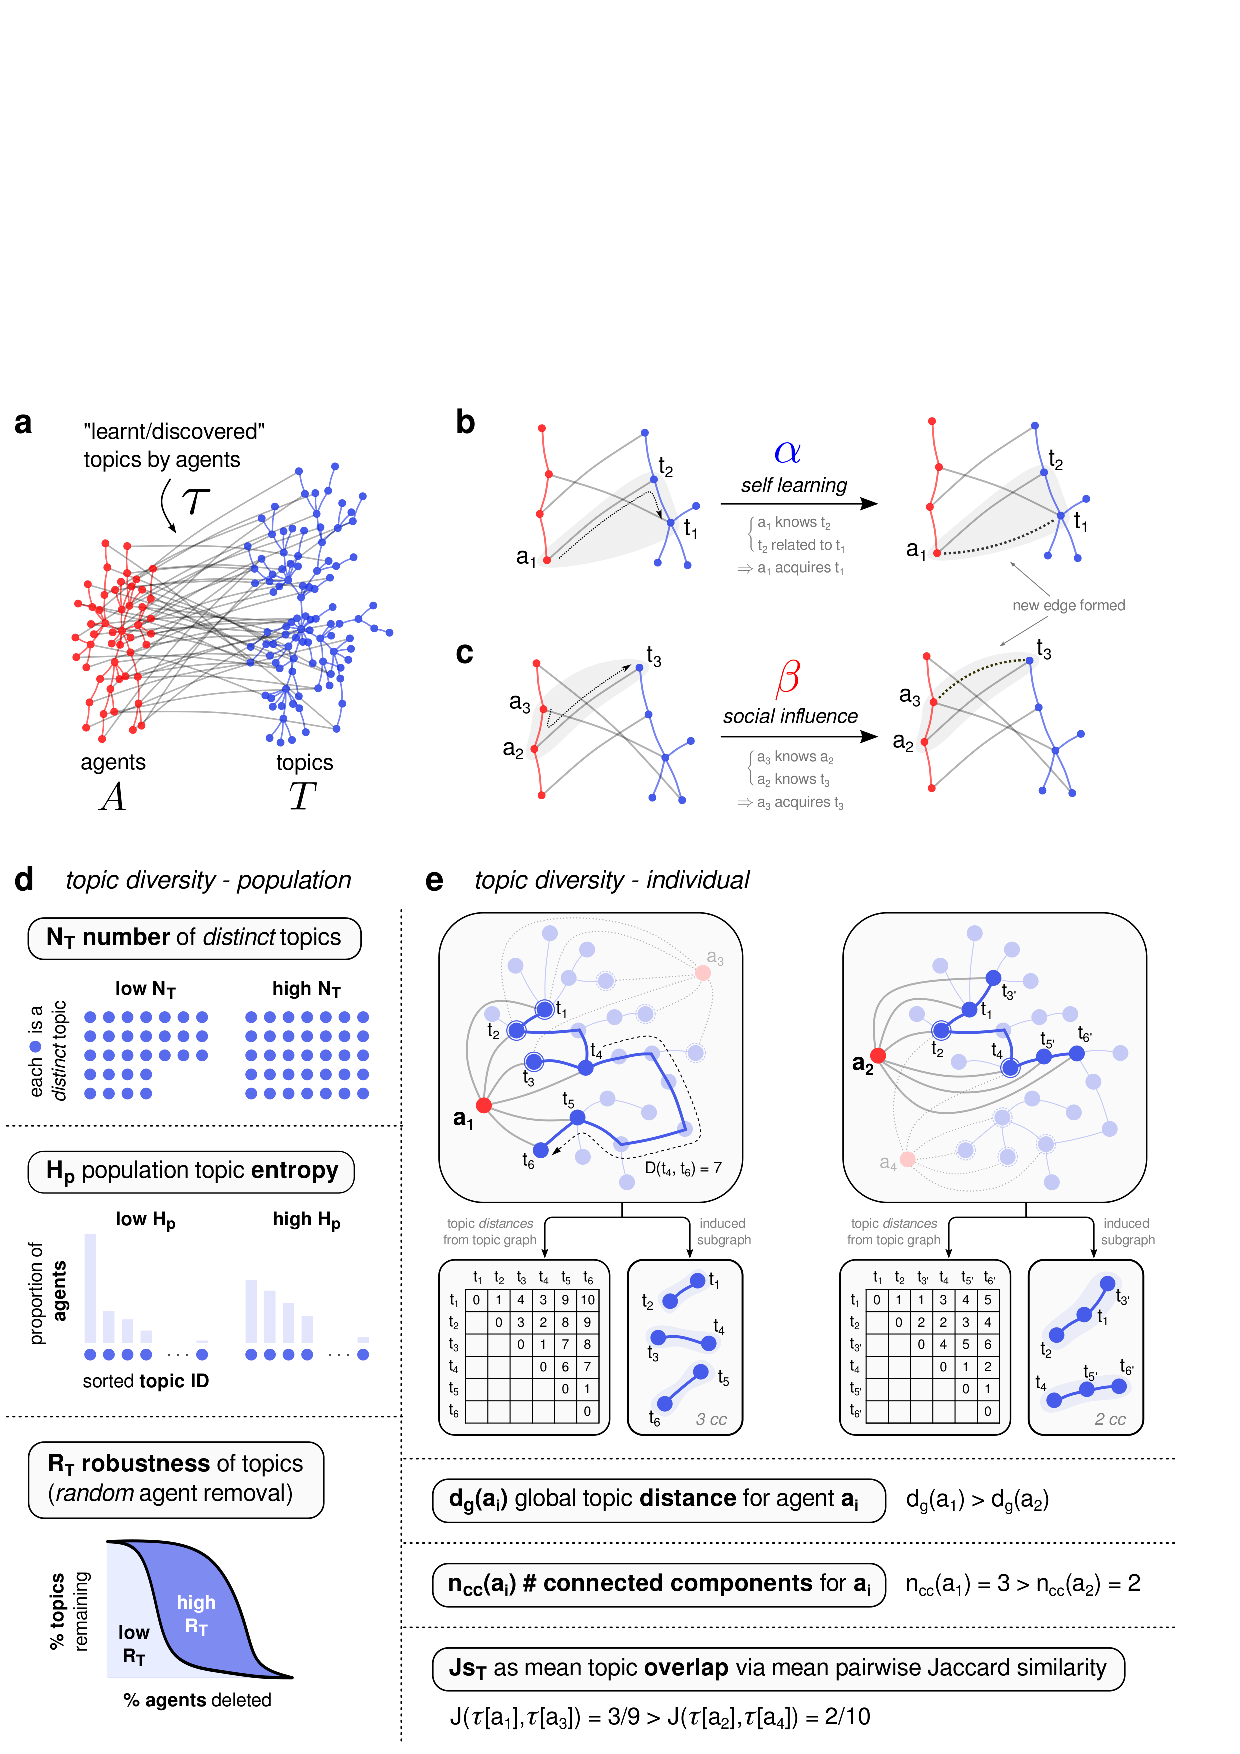
\includegraphics[width=0.95\textwidth,center]{../figures/report/Fig1.pdf}
    \caption{\label{fig:1}
    \textit{Model setup and description of the update process}.
    (\textbf{a}) Illustration of the intralayer agent graph (red) and topic graph (blue) with the interlayer edges (gray) representing the knowledge set of the agents.
    (\textbf{b}) and (\textbf{c}) illustrate the update process either through learning/discovery by related topics ("rabbit-hole") or learning/discovery through friends ("recommender")
    }
\end{figure}

All models considered here are binary undirected graphs. There are $n_a = 200$ agents and $n_t = 1000$ topics. Denote $A$ and $T$ as the symmetric binary adjacency matrices of the agent graph $G_a$ and topic graph $G_t$ respectively (\ref{fig:1}). The bipartite incidence matrix $\tau$ of size $n_t \times n_a$ represents the topics that the agents know about. It is assumed throughout that the intralayer edges are static while the interlayer edges could be ``acquired" through the update process. And once an interlayer edge is acquired, it is assumed to be persistent. At the initial stage, each agent is assigned at most $\tau_0 = 5$ topics with certain probabilities based on the models of the intralayer models (see below). There is also an upper limit topic capacity $\tau_{\mathrm{max}} = 50$ per agent, and the update process is only simulated until $1.2 \tau_{\mathrm{max}} = 60$ time steps. For each parameter set ($\alpha$, intralayer models, interlayer initialization), I ran 5 simulations each. Hopefully in the future I could acquire more computational resources to run more simulations on larger networks (especially for the more realistic graphs built from real-world networks).

\subsubsection*{Update of interlayer edges}

At each time step, at most one new topic is learnt per agent. The agent could acquire new topic edge either through the ``rabbit-hole'' strategy with $\alpha$ probability, by learning about the related topics of things an agent already knows about. On the other hand, with probability $\beta$, an agent could acquire a new topic edge by traversing its neighbors in the agent graph then to the topic graph. See \ref{fig:2} for illustration of these processes. One way to implement this is below.

Define $\psi(X)$ as a column L1 normalization operation on a matrix $X$, meaning each column vector $\vec{x}_i$ of the matrix is normalized to $\vec{x}_i/||\vec{x}_i||_1$. Define the shorthand notation for the Heaviside function as $[x]_{\star} = 1$ if $x > 0$, and $0$ otherwise.

At each time step, the probability matrix $P$ (of same size as $\tau$) with its column vector $\vec{p}_i$ defining the probability agent $a_i$ choosing a new topic. A way to define this probability is:

% \vspace{-1em}
\begin{eqnarray}
    P &=
    \alpha \psi\left(\left[\left[T\tau\right]_{\star} - \tau \right]_{\star}\right) +
    \beta \psi\left(\left[\left[\tau A\right]_{\star} - \tau \right]_{\star}\right)
    \\
    \tau(t+1) &\leftarrow \tau(t) + \mathrm{sample}(P)
\end{eqnarray}

The multiplication steps perform the traversal through neighbors across the intralayer networks. The binarization and subtraction of current $\tau$ simplifies the implementation, to only learn new topics and to balance not being stuck around too popular topics. Additionally, for simplicity here I consider $\beta = 1 - \alpha$ so the process is only defined by $\alpha$. Many other probabilities are ignored as well, for example serendipity (wandering or random discovery of new topics) and forgetting (removal or decrease of strength of interlayer edges). Future implementations should relax these many assumptions for more realistic implementation, and possibly easier to obtain analytical solutions when the nonlinearities are minimized.

\begin{figure}[H]
    \centering
    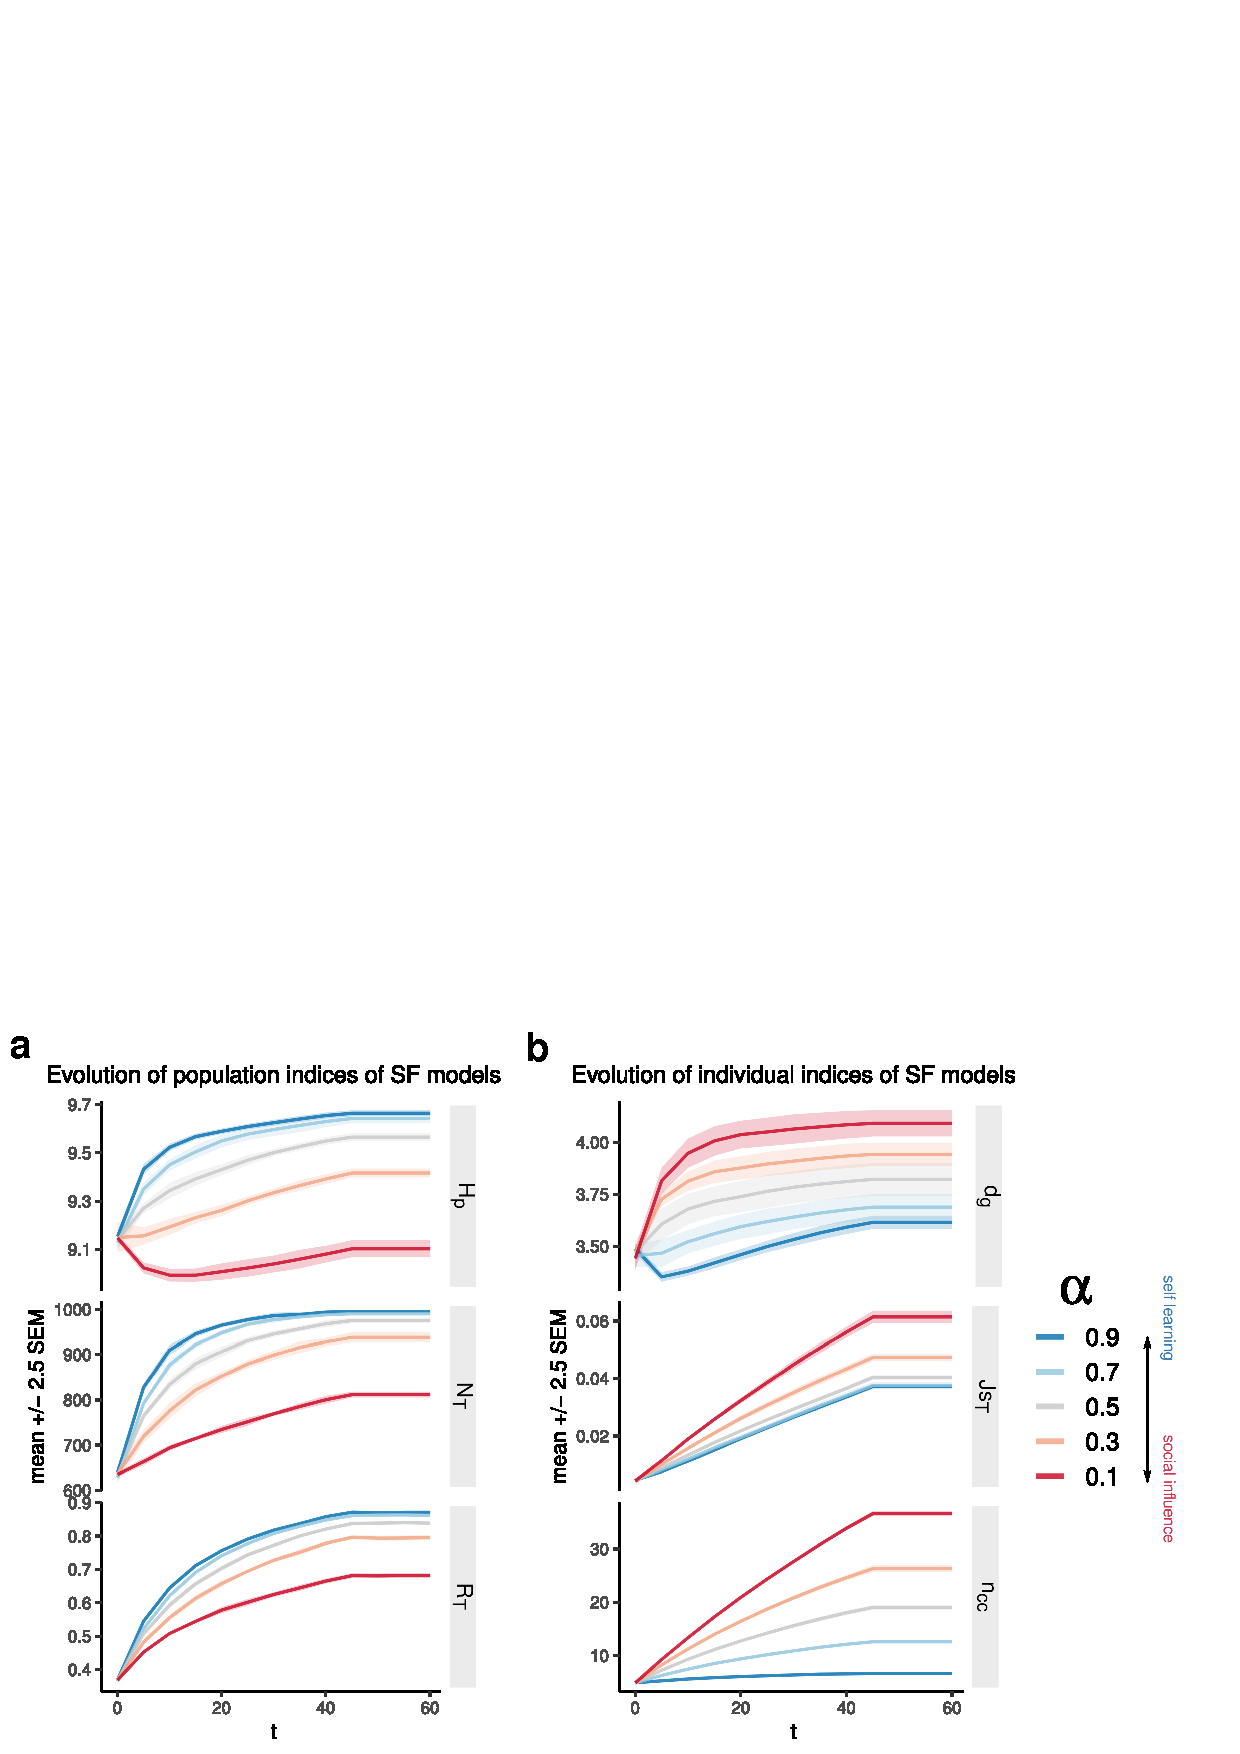
\includegraphics[width=0.95\textwidth,center]{../figures/report/Fig2.pdf}
    \caption{\label{fig:2}
    \textit{Examples of intralayer static model set up}. For simplicity, for all instances, the types of models used are the same for both agent and topic graph.
    (\textbf{a}) Non-block models (PA: preferential attachment, ER: Erdős–Rényi, WS: Watts–Strogatz; see method for more details). (\textbf{b}) Stochastic block models (SBM) with decreasing modularity by increasing the connection probability between members of different groups. There are 10 groups for each intralayer model.
    }
\end{figure}

\subsubsection*{Intralayer random models}

There are different ways to initialize the intralayer networks to match with different empirical results in real social and knowledge networks. For simplicity, the model types and parameters (except only for the number of nodes) are kept the same for agent and topic graphs during each simulation.

\textit{Nonblock models}: The first approach is non-block networks. These include models constructed from preferential attachment models (PA), in which linear PA would lead to a scale-free network with the scaling parameter $\gamma = 3$. I also take into account nonlinear PA models (see \ref{fig:2}a$_1$). I also include comparison with Erdős–Rényi (ER) networks with different connectivity probability (see \ref{fig:2}a$_2$), as well as small-world networks generated with the Watts–Strogatz models (see \ref{fig:2}a$_3$).

\textit{Block models}: Since in real-world networks, there are usually communities (researchers or papers within the same field), I use the stochastic block models (SBM) to emulate this with $k_a = k_t = 10$ groups for both agent and topic networks. A way to manipulate these models is to change the probability of connection within groups ($p_{\mathrm{within}}$) or between groups ($p_{\mathrm{between}}$). For simplicity, I kept the former the same while varying the latter (see \ref{fig:2}). In retrospect, this makes the models denser by increasing the $p_{\mathrm{between}}$. Future simulations should look for ways to balance this.

Future endeavours should take into account real networks, for example from subsampling a Twitter network as the agent graph and Wikipedia network as the topic graph. Another possibility would be to use citation networks, with authors as agents and papers as topics, groups could be subfields or certain modules in the research topics.

\subsubsection*{Interlayer initialization}

Generally at the initialization stage, the probability of connection between a given agent and topic could be the same across topics. However, it is possible that other initialization strategies might bias the results in one way or another. Hence, I introduce two different interlayer initialization strategies, one for \textit{nonblock} intralayer models and one for \textit{block} models. Whenever an initialization method is not mentioned, it is assumed to be the uniform random strategy.

For \textit{nonblock} intralayer models, the probability of connecting to a certain topic could be dependent on its degree in $G_t$. A way to do this is to perform the $\mathrm{softmax}\left(\{d_i\}; \beta_{\sigma}\right)$ on the degrees, basically transforming the degree sequence $\{d_i\}$ to a probability distribution. With $\beta_{\sigma} < 0$ ($\mathrm{SOFTMAX}_1$), low degrees are favored; $\beta_{\sigma} = 0$ is equivalent to random initialization ($\mathrm{SOFTMAX}_2$), while $\beta_{\sigma} > 0$  ($\mathrm{SOFTMAX}_3$) favors high degree topics (\ref{supp:1})

For \textit{block} intralayer models, group correspondence could be used as a strategy for initialization as the number of groups are the same for both graphs. This could be parameterized by $p_{\mathrm{sg}}$ (\ref{supp:2}) as the probability that agents and topics of the same group ID are connected. The chance $p_{sg} = \frac{1}{k_t} = 0.1$ would be equivalent to random initialization.

\subsection{Diversity metric}

\subsubsection*{Population}

Three population indices are defined. First is $N_T$ the number of distinct topics discovered when taking into account all agents' learnt topics (higher would mean more diverse). Second is the topic population entropy $H_p$, which is the Shannon entropy from the discrete probability distribution of all the topics in the population (higher would mean more diverse). Lastly, taken inspiration from ecological bipartitate network stability analysis, robustness can be calculated, by cumulatively removing random agents and observering the number of distinct topics left. The area under this curve is the robustness (higher would mean a lot of agents are needed to be removed to remove a sufficient large proportion of topics).

\subsubsection*{Individual}

Three individual indices are calculated. $d_g$ is the mean distance of the topics in each agent's learnt topics. In other words, if we define $D(t_i,t_j;G_t)$ as the shortest path distance in $G_t$ between $t_i$ and $t_j$, and an agent $a_k$'s topic set as $\tau(a_k)$ then $d_g(a_k) = E\left[D(t_i,t_j;G_t)\right]_{t_i, t_j \in \tau(a_k)}$. Then I take the mean of these distances across off agents of the agent graph. Higher would mean, on average, the agents learn more out of their comfort zone. Another metric is the number connected component $n_{\mathrm{cc}}(a_k)$ of the induced subgraph $G_t(\tau(a_k))$ - higher would mean there are many ``islands'' of topics that the agent knows about, leaning toward generalist trend. Lastly, the pairwise Jaccard similarity between agents' topic sets are calculated $Js_T$, lower would mean higher local diversity on average. Future endeavours should take into account other metrics for local diversity indices (for example local entropies under subsampling of neighbors or nodes within a certain distance).

\subsubsection*{Group}

Additionally, when groups are defined in the block intralayer models, one could also calculate the entropy of the topic group distribution, in both the population sense $H_{\mathrm{gp}}$ and individual sense $H_{\mathrm{gi}}$. More specifically, $H_{\mathrm{gp}}$ is the entropy of the 10 topic groups when taking into account the group identities of all topics learnt by all agents. On the other hand, $H_{\mathrm{gi}}$ is the average entropy of each agent's own topic entropy. These two quantities are different. For example, there could be cases where as a population, $H_{\mathrm{gp}}$ is maximized (all groups uniformly distributed) but $H_{\mathrm{gi}}$ could be 0 (each agent only learns about the topics of the same group, leading individual entropy of 0).

\section{Results}

\subsection{\textit{Nonblock} intralayer models}


\begin{figure}[!ht]
    \centering
    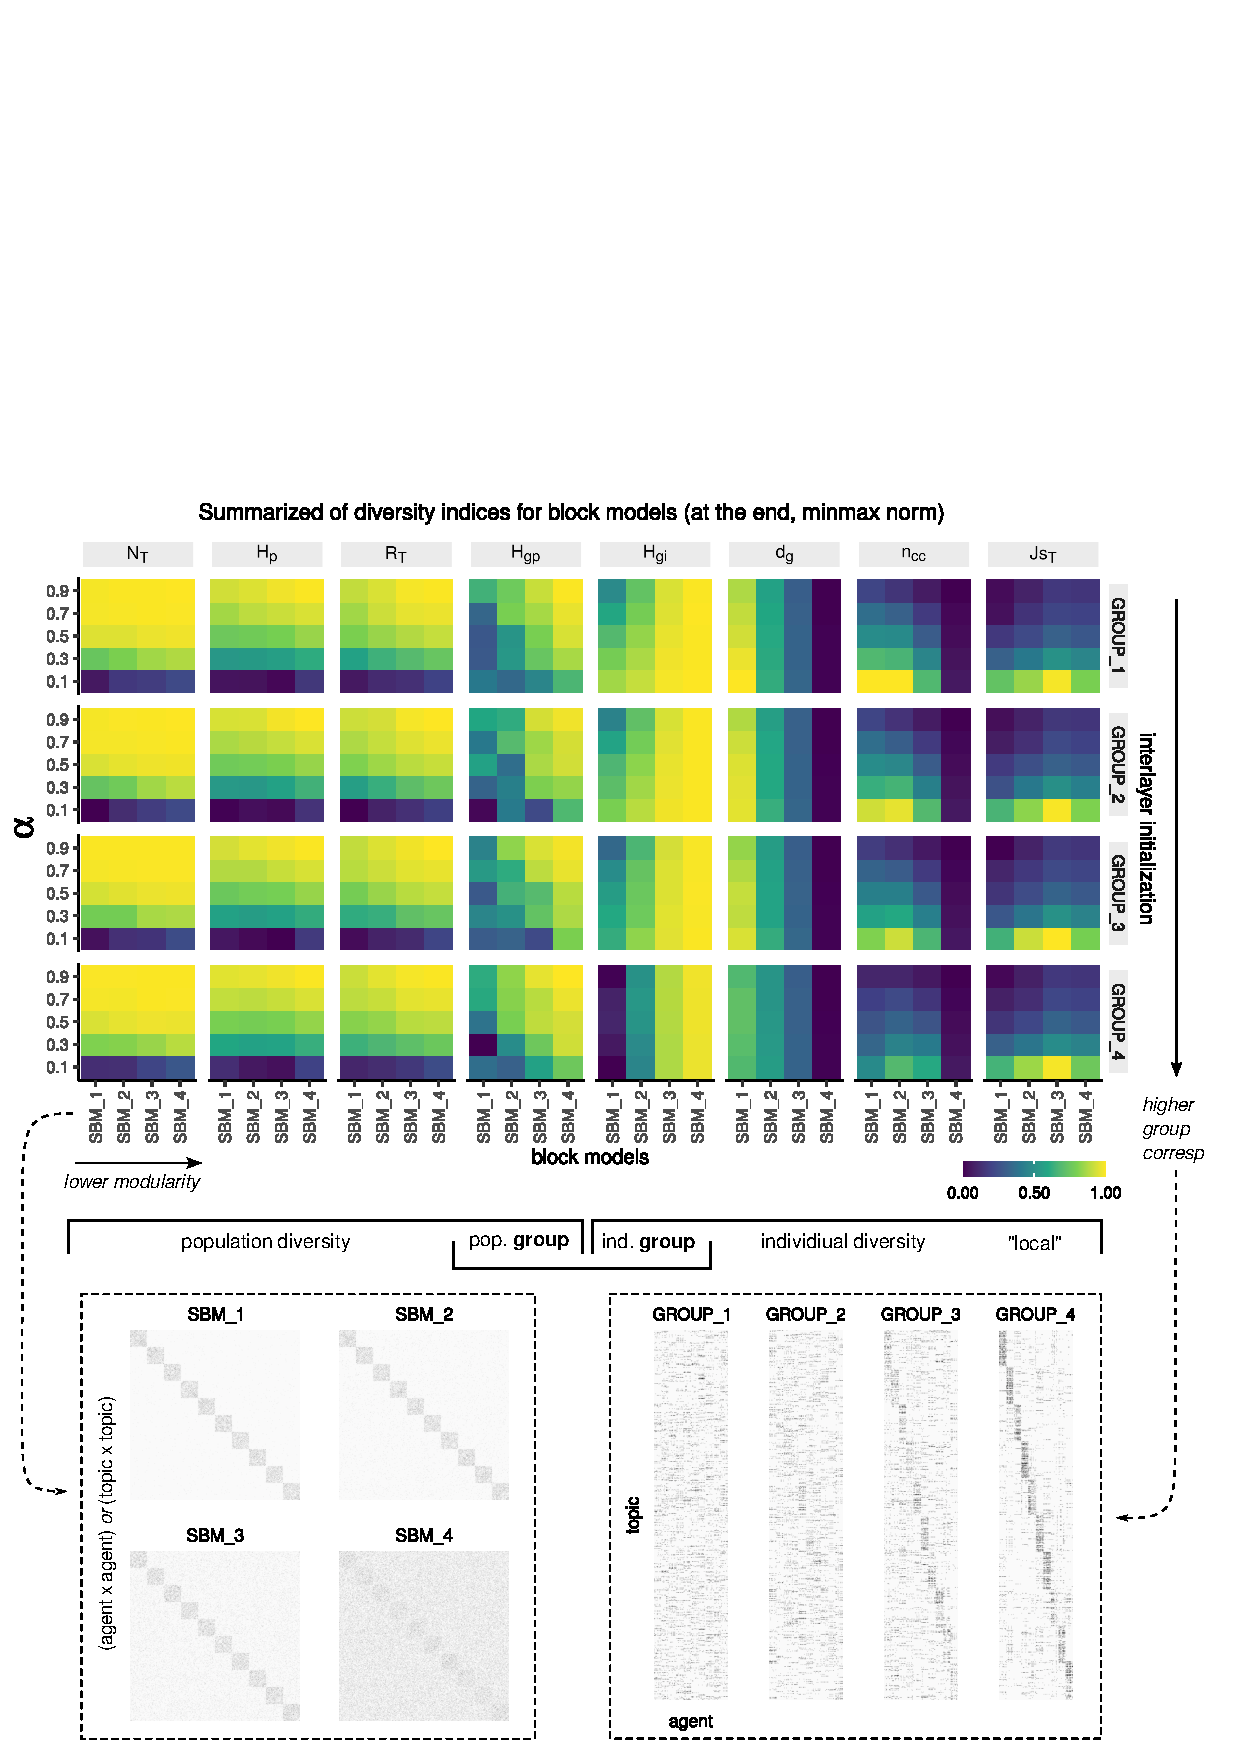
\includegraphics[width=\textwidth]{figures/Fig3.pdf}
    \caption{
    \textit{Summary  of  population  and  individual  diversity  indices  due  to $\alpha$,  across  different  block  models}. Within each heatmap, x-axis shows decreasing modularity of intralayer model (via increasing inter-modular connectivity), y-axis is $\alpha$. The color represents values at the end of the simulations, and min-max normalized within each metric. From left to right are different diversity metrics. From top to bottom are different group correspondence initialization strategies.
    }
    \label{fig:3}
\end{figure}


The changes of the different diversity metrics for the scale-free networks ($PA_2$) are shown in \autoref{fig:3} as an example to illustrate the tradeoff effect of the ``rabbit-hole'' versus ``recommender'' probability on the population and individual diversity.

Generally, topic population diversity increases with $\alpha$ in terms of the topic entropy $H_g$ and number of topics $N_T$. Through learning/discovery through time, low $\alpha$ could still achive better population diversity. However, it does not seem likely for the worst case considered here, where entropy does not even increase pass its initial value. The initial decrease of $H_g$ when $\alpha = 0.1$ is because the agents start learning from each other, hence temporarily creating bias towards some topics, leading to decrease of entropy. It must be noted here that the entropies are already high initially due to initialization. However, taking the trends of both $N_T$ and $H_g$ into account, it is confident to say that higher $\alpha$ improves topic population diversity. Additionally, higher $\alpha$ leads to more robust retainment of the topics under random agent removal (i.e. higher $R_T$).

On the other hand, topic individual diversity usually decreases based on the chosen metrics. Increased $\alpha$ leads to decreased mean learnt topics distance $d_g$ and number of components $n_{\mathrm{cc}}$ in the induced subgraphs. Intuitively, lower $\alpha$ would allow the agents to access topics out of their comfort zone easier, hence their own subgraph of topics tend to be more generalist, whereas higher $\alpha$ leads to more specialization. Lastly, at the local level $Js_T$, lower $\alpha$ leads to more similarity between neighbors, hence lower local diversity.

These trends are quite consistent across different considerations of non-block models (\autoref{fig:4}). Increasing in $\alpha$ leads to higher topic population diversity ($N_T, H_P$), robustness ($R_T$) and local diversity $Js_T$. On the other hand, such increases tend to result in loss of topic individual diversity ($d_g$, $n_cc$). When taking into account degree-dependent initialization strategies (\autoref{supp:1}), favoring more obscure topics leads to the same trend as random initialization, though small effects when $\alpha$ is small (first 2 rows in \autoref{supp:3}). However, initially favoring more popular topics actually would be detrimental generally across all population, local and diversity, especially for those networks generated by preferential attachments (PA) models, possibly the learning gets ``stuck'' around the nodes around those population ones (last row in \autoref{supp:3})

\begin{figure}[!ht]
    \centering
    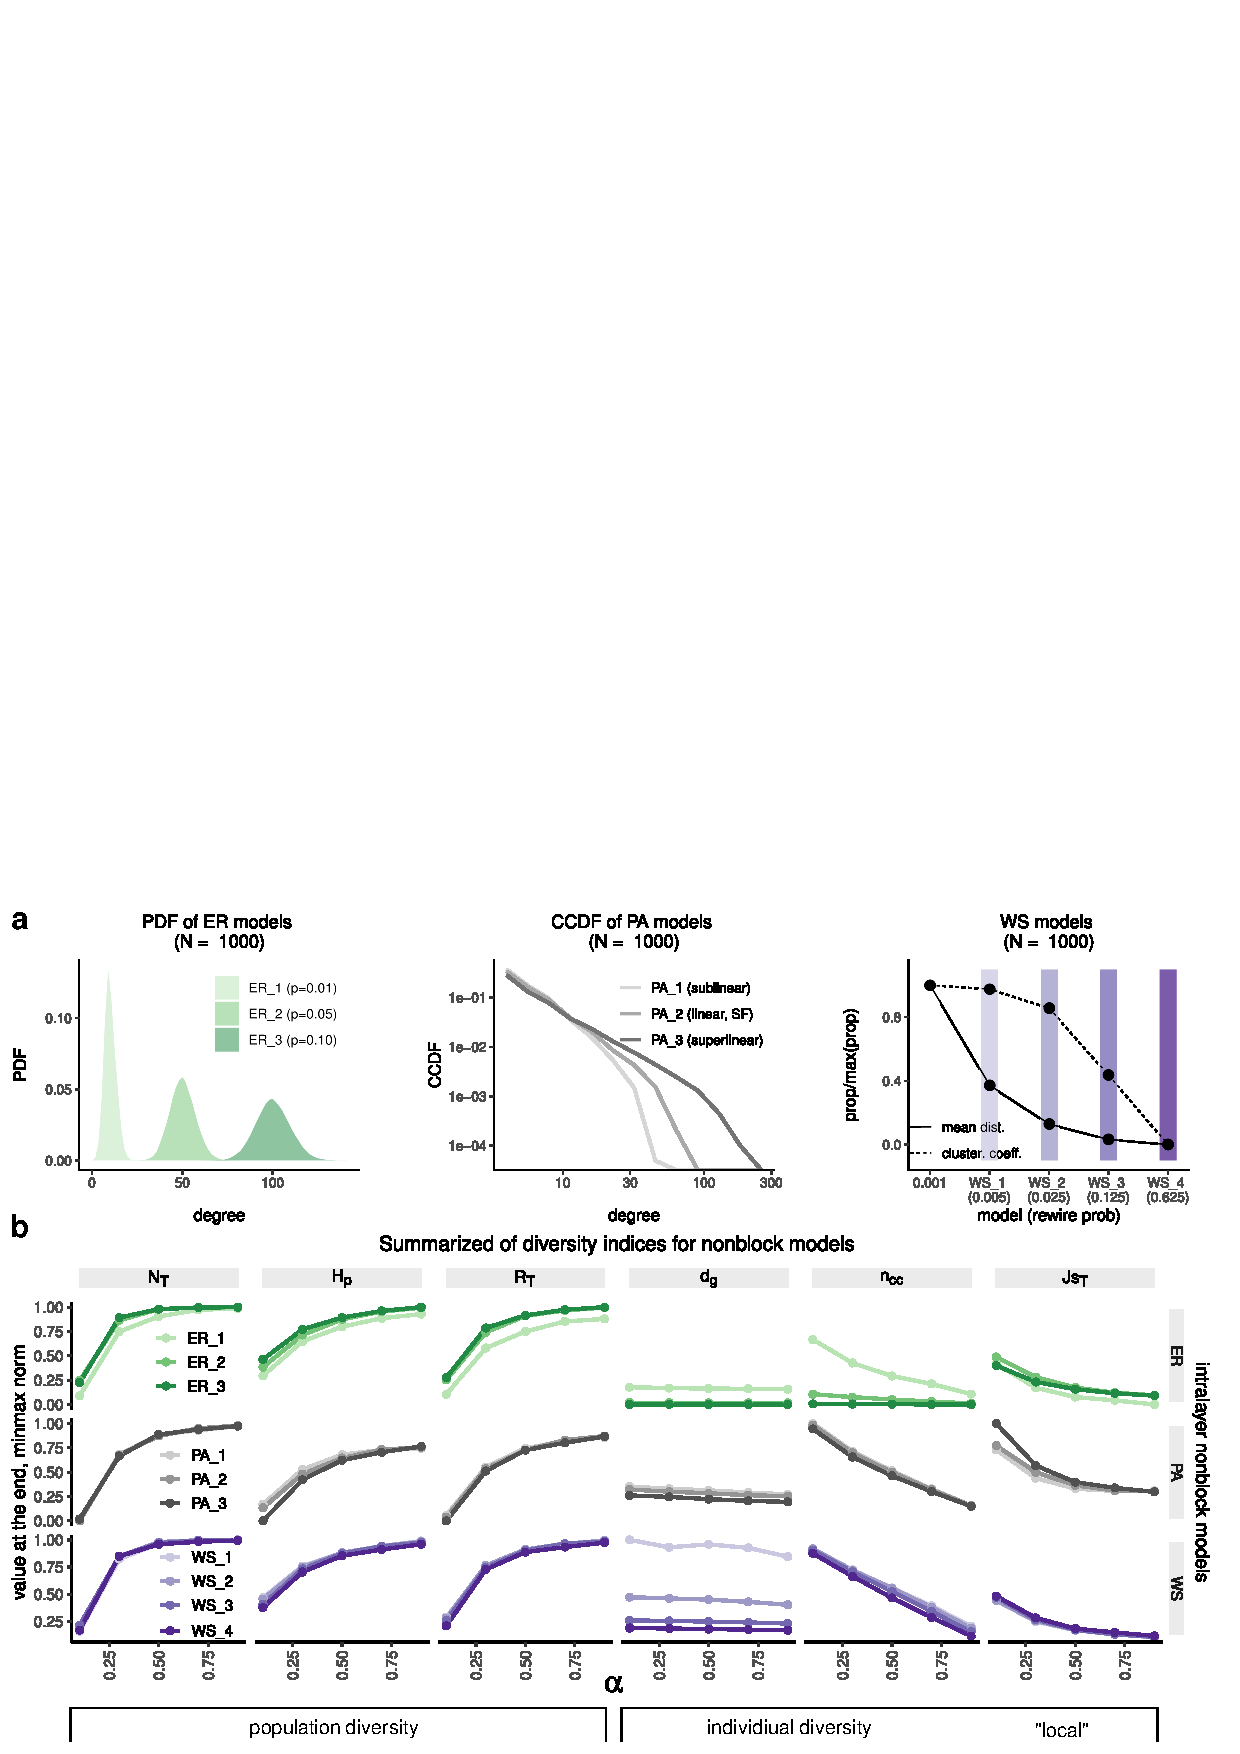
\includegraphics[width=\textwidth]{figures/FigS1.pdf}
    \caption{\label{fig:4}
    \textit{Summary of population and individual diversity indices due to $\alpha$, across different nonblock models (with random initialization)}. The values here are at the end of the simulation, and min-max normalized within each metric (panels from left to right, see text and \ref{fig:3} for description of these different definitions). The different models are shown by colors and panels from top to bottom (see also \ref{fig:2} for correspondence of colors).
    }
\end{figure}

In summary, in non-block intralayer models, higher $\alpha$ leads to higher topic diversity in a local and population context, but lower individual topic diversity. Initialization favoring more popular topics seems to have a negative effect on these different metrics.


\subsection{\textit{Block} intralayer models and topic group diversity}

As real-world networks usually contain communities within them, I use the stochastic block models (SBM) to observe how diversity indices change due to $\alpha$ and network modularity. Generally the trends for population diversity and robustness during the simulation are similar from previously discussed (\autoref{supp:4}). The trends as a function of model modularity do not seem to differ much either (however the final values do show some differences, and will be discussed later). Looking at the group population entropy $H_{\mathrm{gp}}$ (\autoref{fig:5}a), only when the networks are less modular do such values show a difference, albeit very small. In particular, only when $\alpha$ is very low that such a disadvantage could be visibly inspected (very low $\alpha$ basically leads to learning in groups).

In the individual perspective (\autoref{fig:5}b), group modularity actually helps with diversity indices $d_g$ and $n_{\mathrm{cc}}$, possibly because there are few long-range links. The trends for local diversity are roughly similar and not affected much by group modularity. However, their final values do show some difference (will be discussed later). Additionally, instead of only looking at topic group diversity in the population sense, one could also inspect it in the individual perspective. On average (panel a, top), for more modular intralayer networks, lower $\alpha$ benefits topic group diversity in the agents, because the agents would have higher chance to learn out of their own comfort zone, especially if their initial topics belong to the same groups. With decreasing group modularity, these differences between $\alpha$ do not seem to matter any more.

\begin{figure}[H]
    \centering
    \includegraphics[width=0.85\textwidth,center]{../figures/report/Fig5.pdf}
    \caption{\label{fig:5}
    \textit{Changes of group diversity indices} (\textbf{a}) \textit{and of individual diversity indices} (\textbf{b}) \textit{of the stochastic block intralayer models} \textit{due to} $\alpha$. $H_{\mathrm{gi}}$: topic individual entropy; $H_{\mathrm{gp}}$: topic population entropy. From left to right, the models are designed to have decreasing modularity (see \autoref{fig:2}). See also \autoref{fig:3} and text for descriptions of individual diversity metrics.
    }
\end{figure}

Inspecting the end values of these different metrics in \autoref{fig:6} taken into account group-correspondence initialization strategies reveal these effects more clearly.

More specifically, higher $\alpha$ and lower intralayer modularity leads to high population topic diversity and robustness ($N_T, H_p, R_T$), whereas group correspondence initialization does not seem to have pronounced effects. Group modularity benefits the individual diversity ($d_g, n_{\mathrm{cc}}$) but high initial group-correspondence would counter such effects. For local level, group-correspondence does not seem to affect $Js_T$ visibly. However, generally higher $\alpha$ and higher model modularity tends to decrease topic similarity, hence increasing local diversity.

When we start to consider group entropies, generally low group modularity increases both topic group population ($H_{\mathrm{gp}}$) and individual ($H_{\mathrm{gi}}$). High initial correspondence though seems to benefit group population diversity (although such benefits may be small, see \autoref{fig:5}), it seems to decreases  group individual diversity.

In summary, with consideration of intralayer block models, higher $\alpha$ still benefits more for population diversity and robustness, but not so much with group population diversity. High network modularity may hurt population diversity, regardless of initial group-correspondence. On the other hand, lower $\alpha$ is more beneficial for individual indices, including group individual diversity, but either low network modularity or higher group correspondence would tend to be harmful for these metrics. At the local level, higher $\alpha$ and high network modularity tends to be more beneficial for decreasing similarity between agents.

\begin{figure}[H]
    \centering
    \includegraphics[width=0.95\textwidth,center]{../figures/report/Fig6.pdf}
    \caption{\label{fig:6}
    \textit{Summary  of  population  and  individual  diversity  indices  due  to $\alpha$,  across  different  block  models}. Within each panel, x-axis shows decreasing modularity of intralayer model, y-axis is $\alpha$ while the color represents values here at the end of the simulation, and min-max normalized within each metric. From left to right are different diversity metrics (see text for more information). From top to bottom are different group correspondence initialization strategies (top is equivalent to a random initialization; see \autoref{supp:2} for example)
    }
\end{figure}

\section{Discussion}

In conclusion, with this simple toy model of topic discovery and a simple update rule depending on the probability of traversing through neighbors of bipartite networks, some interesting results are obtained. First of all, increasing in $\alpha$ (self-learning, traversing through interlayer edges first) leads to higher topic population diversity and robustness in various random models for the intralayer networks, including blocks and non-block models. However, such increase has drawbacks when looking at topic individual diversity, as it reduces the chance for the agent nodes to acquire interlayer edges from topics that are usually ``out-of-their-comfort-zone''. Traversing through intralayer edges first ($\beta$ route) would better benefit individual diversity.

When groups are considered in the intralayer networks, group modularity may hurt the population diversity (though some only by a little) and more apprently for group individual entropy, though interestingly more beneficial for individual indices through the lense of graph distances and components. Although initial group correspondence does not have much effects on the population diversity, it has a dramatic drawback at  the individual level (both entropy and graph metrics).

Though there are interesting results in a theoretical sense as a toy model, there are quite many limitations of the current model. Future studies should relax the assumptions made here and test out different versions of the models, for example inclusion of directed weighted edges (strengths could imply confidence in knowledge in $\tau$), non-persistent interlayer edges, different update probabilities (serendipity, forgetting, strengthing, ...), the cost of learning new subjects, delays in acquiring new knoweldge, different versions of the update equation. Furthermore, future endeavours should take into account performing the update process in real networks, which could be constructed using, as an example, the citation networks (agents as authors, papers as topics, groups as fields or subfields).

Additionally, even within the simulations already generated by this project, there are other directions for further explorations, including examination of the modularity changes in the bipartite $\tau$ or in the projected topic graphs (for example, low $\beta$ might start to create communities as evidenced by high Jaccard similarity), the distribution of specificialists and generalists, as well as calculation of nestedness (due to the defined maximum capacity $\tau_{\mathrm{max}}$, the density of the networks would already be controlled). Furthermore, due to the assumption of persistent interlayer edges, it is possible to characterize properties of persistent homlogy of the networks (or the projected version).

In a bigger picture, regardless of questions about information or diversity, how might the process laid out by this model be relevant to other systems? Due to the simplicity set out by the model and the update process, there could be some biological interpretations, though quite loosely and to be taken lightly. For example, in an ecological perspective, one could consider the agent graph as species with links as certain phenotypic/genotypic similarity, and the topic graph as the different environments with links as environmental similarity. The interlayer edges would represent adaptation of a given species to a given environment. The $\alpha$ route would, in a sense, be analogous to adaptation to new environments that share certain similarity with already-adaptated environments. On the other hand, the $\beta$ route could be adaptation to a new environment that the animal has never been in, yet in nature there already exists similar species that has adaptated to such environment, hence such new adaptation is probable.

Another example can be from the neuroscience perspective, albeit in an oversimplified fashion and possibly biologically implausible. However, as a thought model, the agent graph could be neurons with links between them as correlations between them (either structurally via synaptic connections or functionally through activity). The topic graph could be inputs, in which the intralayer edges could represent either coincidence between these different types of inputs or similarity between them. The interlayer edges could represent which inputs a given neuron could code for. The update process shares some inspiration from associative learning. The $\alpha$ route may represent neurons acquire new inputs to code for due to co-occurence of inputs or just because the inputs are sufficiently similar. The $\beta$ route could be because the neuron gets recruited into the engram encoded for a certain object or abstract concept due to the correlative activity with another neuron that already codes for such object.


% \printbibliography

% \section{Acknowledgement}

I would like to thank Dr. Mercedes Pascual and Dr. Sergio A. Alcala Corona, along with every one in the Network of Ecology and Evolution class, and my friend Poojya Ravishankar, for the discussion and feedbacks on this toy model.

% \section{Supporting information}

\subsection*{Code and data availability}

Current code repository lies here: \url{https://github.com/tuanpham96/topic-diversity} (some updates might be a bit slow push up as I'm in the middle or reorganization). The data are simulations (hence quite large), so I will not be able to make them available straight on Github. However, I'm happy to share them.

\subsection*{Supplementary figures}

\setcounter{figure}{0}
\renewcommand{\thefigure}{S\arabic{figure}}

\begin{figure}[!ht]
    \centering
    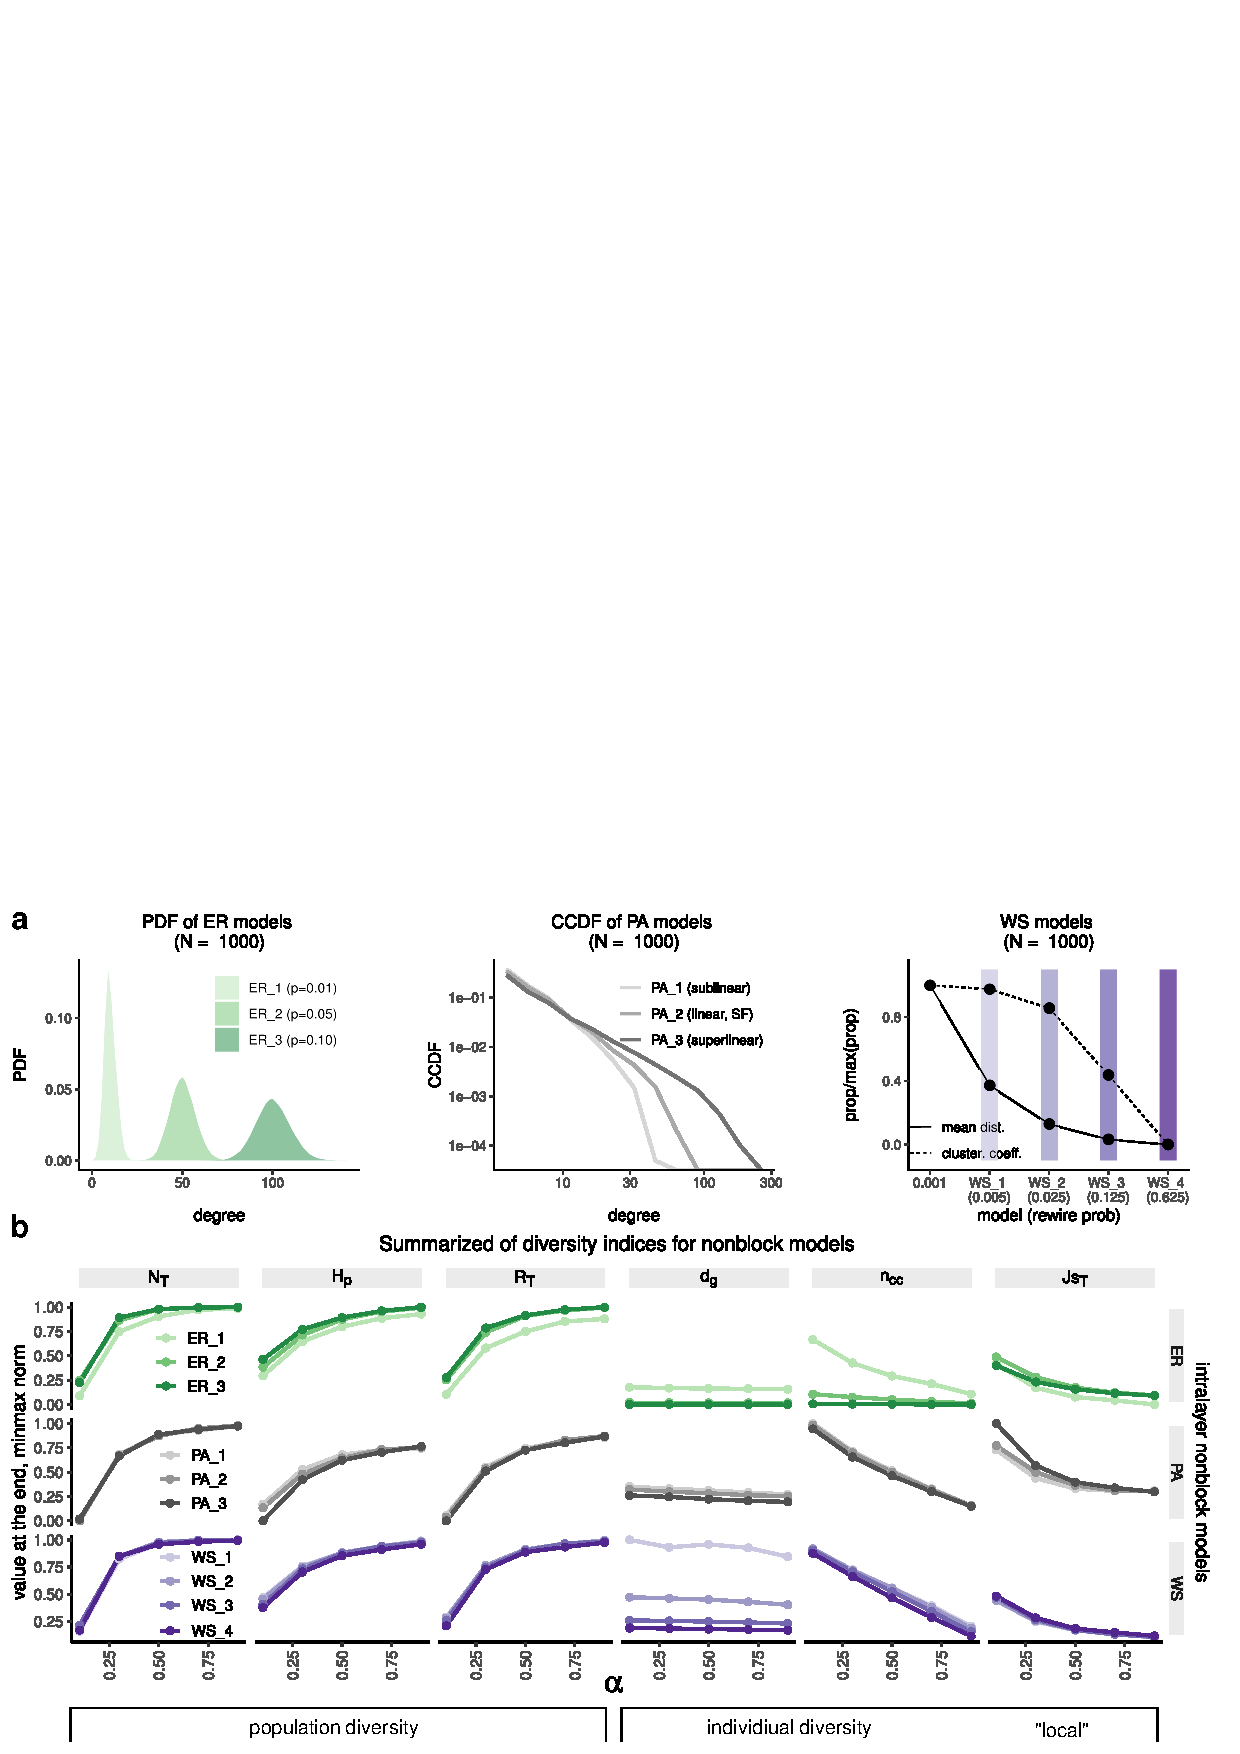
\includegraphics[width=0.9\textwidth]{figures/FigS1.pdf}
    \caption{
    \textit{Variations of nonblock intralayer models}.
    (\textbf{a}) Set up of nonblock models. \texttt{PA}: preferential attachment, \texttt{ER}: Erdős–Rényi, \texttt{WS}: Watts–Strogatz (\textbf{Sect. \ref{sec:method-model}})
    (\textbf{b}) Changes of diversity indices for these models as a function $\alpha$ (\textbf{Sect. \ref{sec:method-diversity}})
    }
    \label{supp:1}
\end{figure}

\begin{figure}[H]
    \centering
    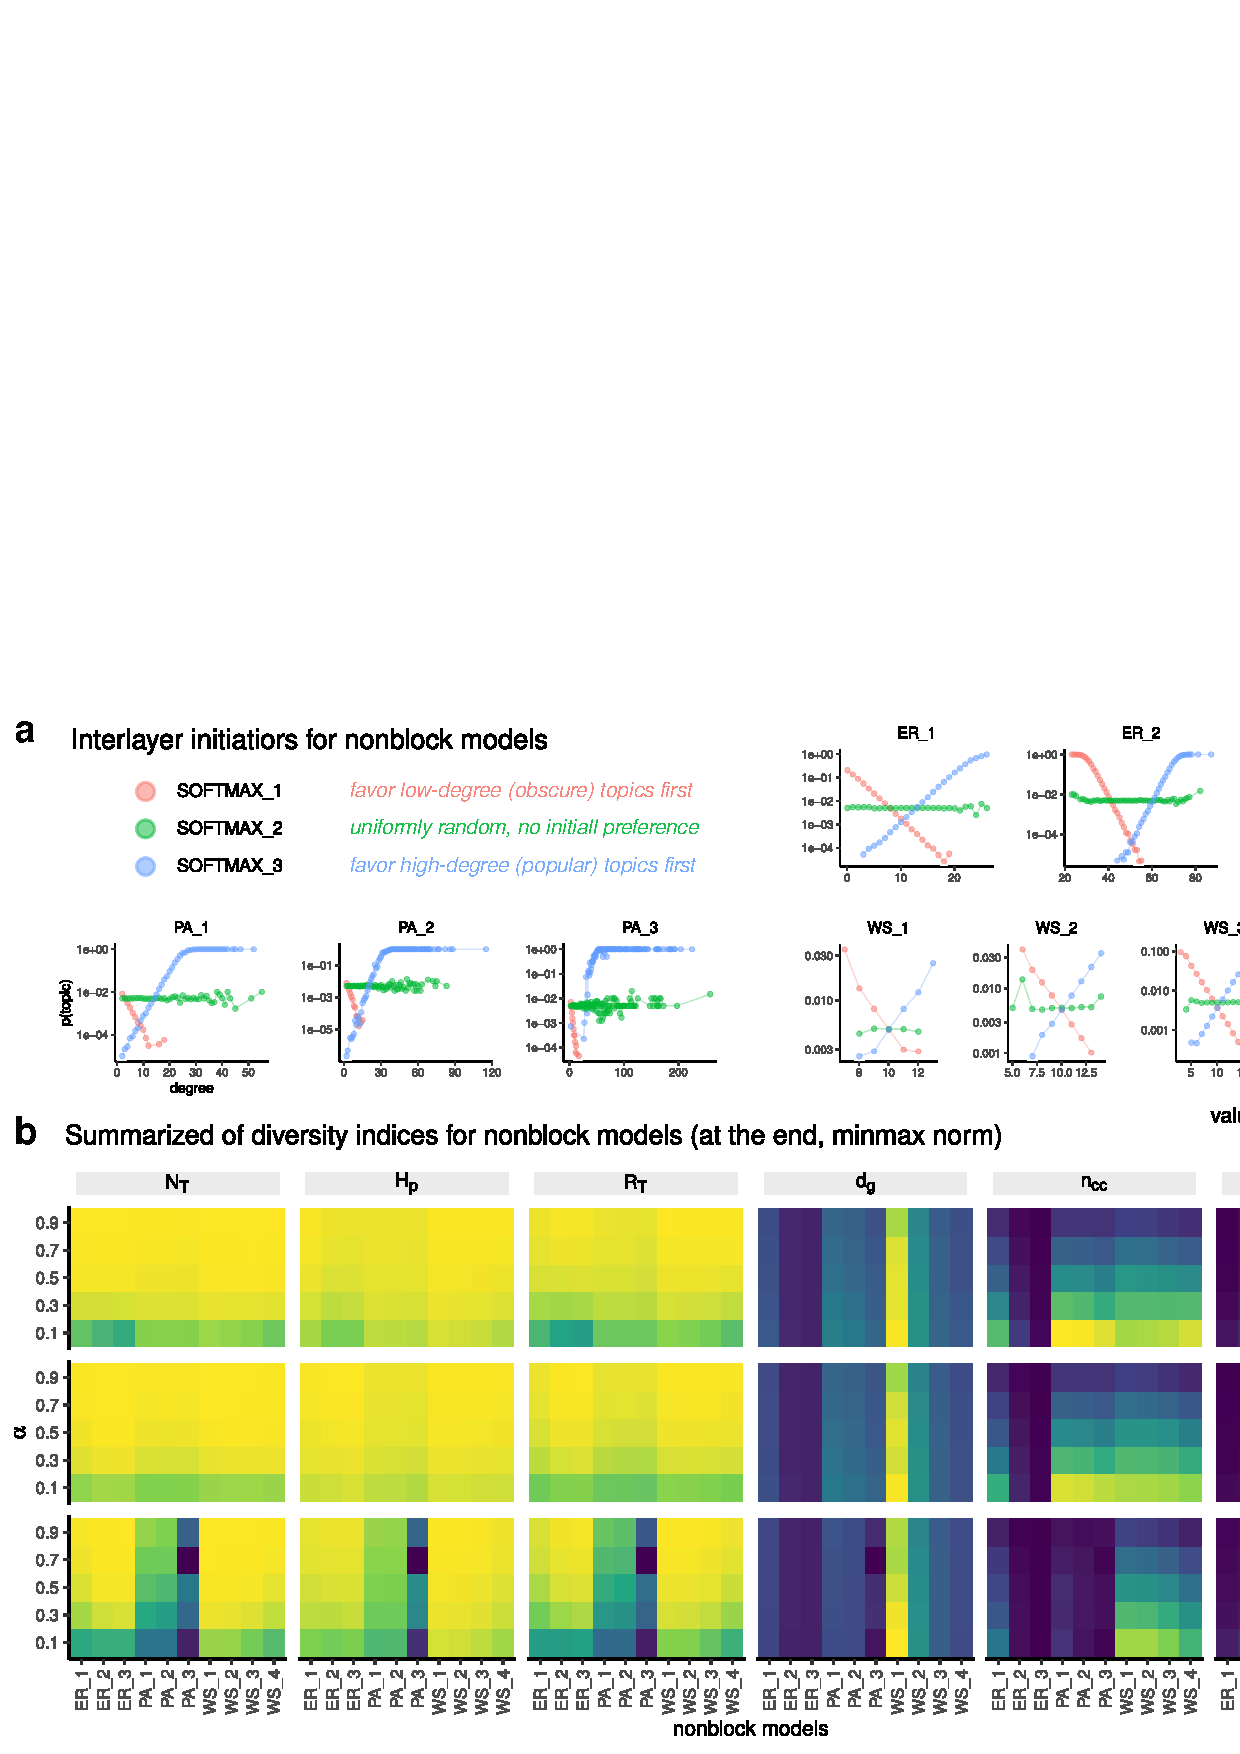
\includegraphics[width=0.5\textwidth,center]{../figures/report/FigS2.pdf}
    \caption{\label{supp:2}
    \textit{Different group correspondence initialization strategies for intralayer block models}
    }
\end{figure}

\begin{figure}[!ht]
    \centering
    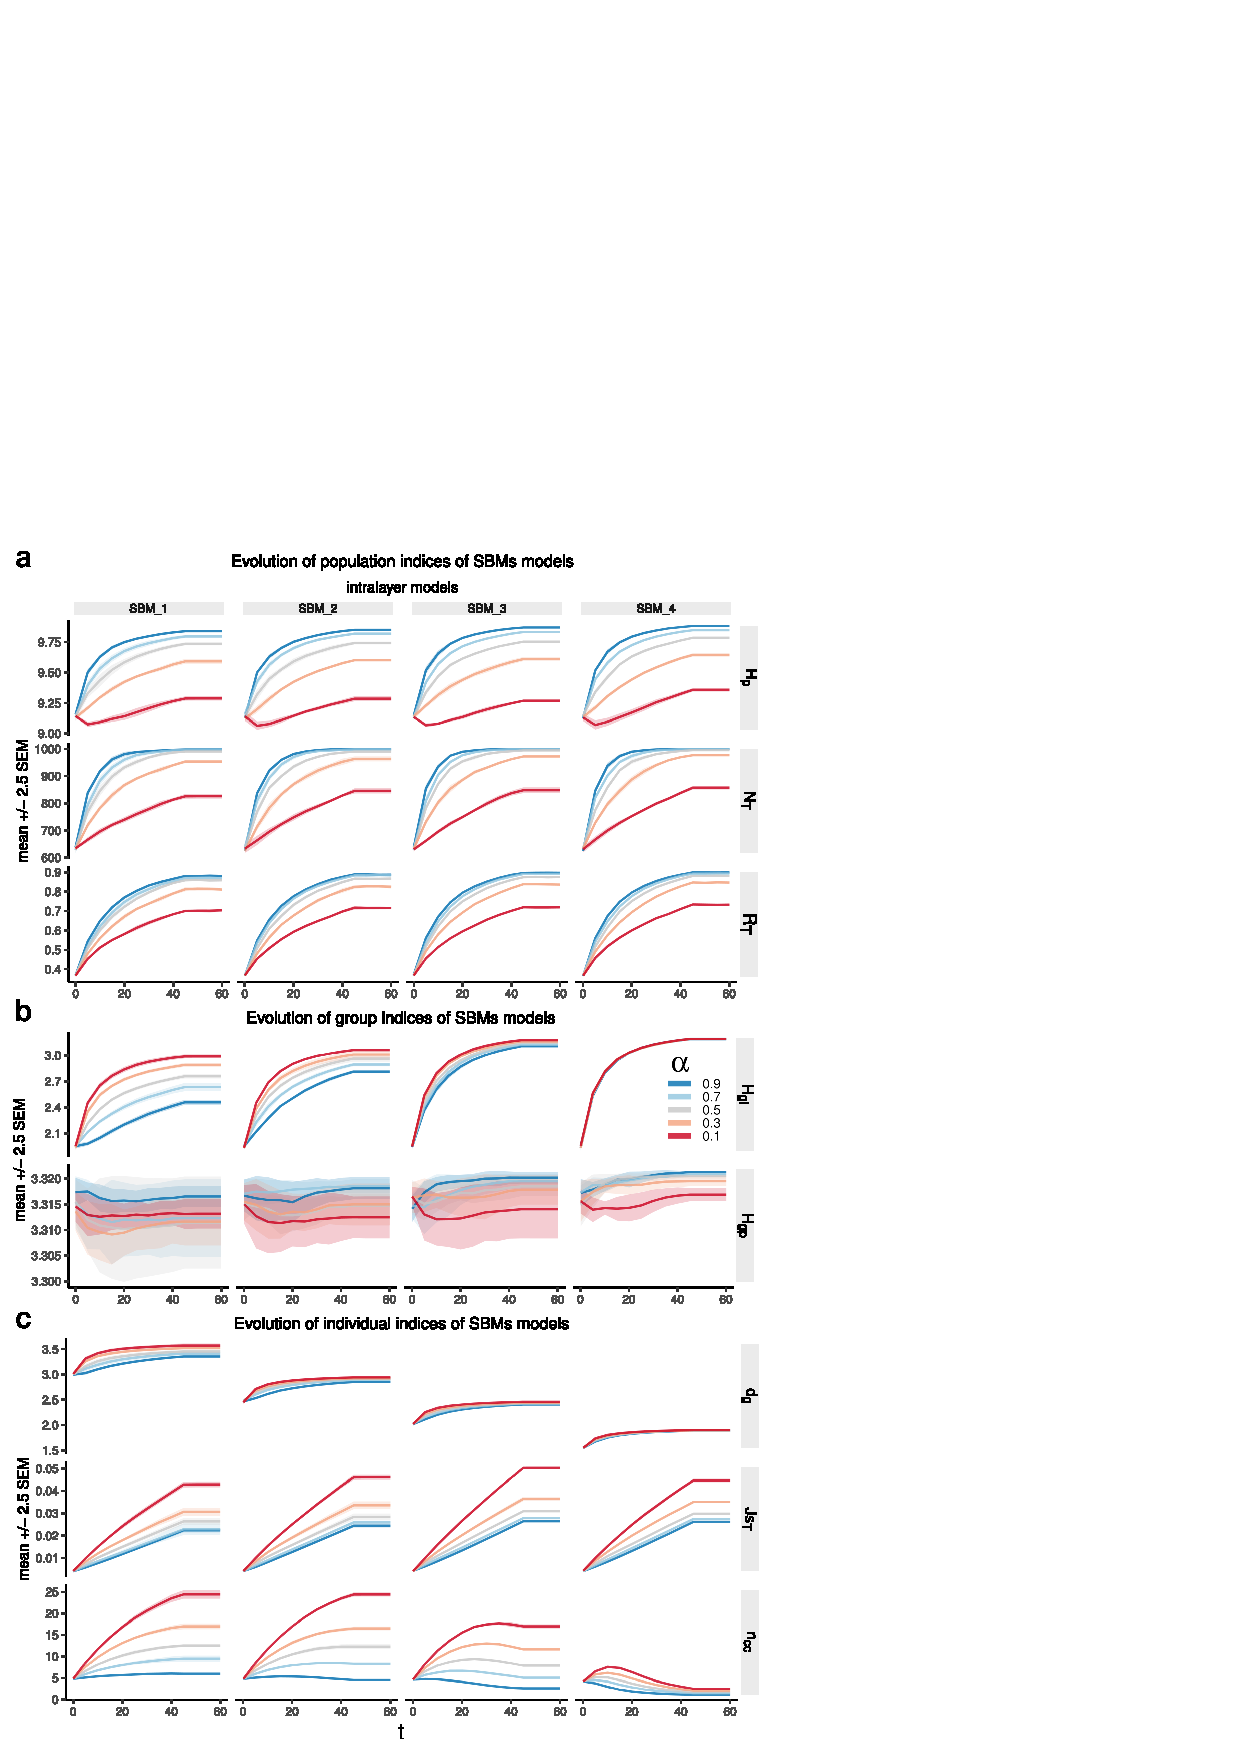
\includegraphics[width=0.85\textwidth]{figures/FigS3.pdf}
    \caption{
    \textit{Changes of population diversity indices} (\textbf{a})\textit{, group diversity indices} (\textbf{b}) \textit{and individual diversity indices} (\textbf{c}) \textit{for the stochastic block intralayer models} \textit{due to} $\alpha$.
    }
    \label{supp:3}
\end{figure}

\begin{figure}[H]
    \centering
    \includegraphics[width=0.95\textwidth,center]{../figures/report/FigS4.pdf}
    \caption{\label{supp:4}
    \textit{Changes of population diversity indices of the stochastic block intralayermodels  due  to $\alpha$}
    }
\end{figure}



\end{document}
